\documentclass[
a4paper,
oneside,
10pt,
fleqn,
headsepline,
toc=listofnumbered, 
bibliography=totocnumbered]{scrartcl}

% deutsche Trennmuster etc.
\usepackage[T1]{fontenc}
\usepackage[utf8]{inputenc}
\usepackage[english, ngerman]{babel} % \selectlanguage{english} if  needed
\usepackage{lmodern} % use modern latin fonts

% Custom commands
\newcommand{\AUTHOR}{Armend Lesi \& Marco Endres}
\newcommand{\INSTITUTE}{Hochschule für Technik Rapperswil}
\newcommand{\LICENSEURL}{https://en.wikipedia.org/wiki/Beerware}
\newcommand{\LICENSE}{
"THE BEER-WARE LICENSE" (Revision 42):
Armend Lesi \& Marco Endres wrote this file. As long as you retain this notice you
can do whatever you want with this stuff. If we meet some day, and you think
this stuff is worth it, you can buy me a beer in return.
}

% Jede Überschrift 1 auf neuer Seite
\let\stdsection\section
\renewcommand\section{\clearpage\stdsection}

% Multiple Authors
\usepackage{authblk}

% Include external pdf
\usepackage{pdfpages}

% Layout / Seitenränder
\usepackage{geometry}

% Inhaltsverzeichnis
\usepackage{makeidx} 
\makeindex

\usepackage{url}
\usepackage[pdfborder={0 0 0}]{hyperref}
\usepackage[all]{hypcap}
\usepackage{hyperxmp} % for license metadata

% Glossar und Abkürzungsverzeichnis
\usepackage[acronym,toc,nopostdot]{glossaries}
\glossarystyle{altlist}
\usepackage{xparse}
\DeclareDocumentCommand{\newdualentry}{ O{} O{} m m m m } {
	\newglossaryentry{gls-#3}{
		name={#4 : #5},
		text={#5\glsadd{#3}},
		description={#6},
		#1
	}
	\makeglossaries
	\newacronym[see={[Siehe:]{gls-#3}},#2]{#3}{#4}{#5\glsadd{gls-#3}}
}
\makeglossaries

% Mathematik
\usepackage{amsmath}
\usepackage{amssymb}
\usepackage{amsfonts}
\usepackage{enumitem}

% Images
\usepackage{graphicx}
\graphicspath{{images/}} % default paths

% Boxes
\usepackage{fancybox}

%Tables
\usepackage{tabu}
\usepackage{booktabs} % toprule, midrule, bottomrule
\usepackage{array} % for matrix tables

% Multi Columns
\usepackage{multicol}

% Header and footer
\usepackage{scrlayer-scrpage}
\setkomafont{pagehead}{\normalfont}
\setkomafont{pagefoot}{\normalfont}
\automark*{section}
\clearpairofpagestyles
\ihead{\headmark}
\ohead{\AUTHOR}
\cfoot{\pagemark}

% Pseudocode
\usepackage{algorithmic}
\usepackage[linesnumbered,ruled]{algorithm2e}

% Code Listings
\usepackage{listings}
\usepackage{color}
\usepackage{beramono}

\definecolor{bluekeywords}{rgb}{0,0,1}
\definecolor{greencomments}{rgb}{0,0.5,0}
\definecolor{redstrings}{rgb}{0.64,0.08,0.08}
\definecolor{xmlcomments}{rgb}{0.5,0.5,0.5}
\definecolor{types}{rgb}{0.17,0.57,0.68}

\lstdefinestyle{visual-studio-style}{
	language=[Sharp]C,
	columns=flexible,
	showstringspaces=false,
	basicstyle=\footnotesize\ttfamily, 
	commentstyle=\color{greencomments},
	morekeywords={partial, var, value, get, set},
	keywordstyle=\bfseries\color{bluekeywords},
	stringstyle=\color{redstrings},
	breaklines=true,
	breakatwhitespace=true,
	tabsize=4,
	numbers=left,
	numberstyle=\tiny\color{black},
	frame=lines,
	showspaces=false,
	showtabs=false,
	escapeinside={£}{£},
}

\definecolor{DarkPurple}{rgb}{0.4, 0.1, 0.4}
\definecolor{DarkCyan}{rgb}{0.0, 0.5, 0.4}
\definecolor{LightLime}{rgb}{0.3, 0.5, 0.4}
\definecolor{Blue}{rgb}{0.0, 0.0, 1.0}

\lstdefinestyle{cevelop-style}{
	language=C++,  
	columns=flexible,
	showstringspaces=false,     
	basicstyle=\footnotesize\ttfamily, 
	keywordstyle=\bfseries\color{DarkPurple},
	commentstyle=\color{LightLime},
	stringstyle=\color{Blue}, 
	escapeinside={£}{£}, % latex scope within code      
	breaklines=true,
	breakatwhitespace=true,
	showspaces=false,
	showtabs=false,
	tabsize=4,
	morekeywords={include,ifndef,define},
	numbers=left,
	numberstyle=\tiny\color{black},
	frame=lines,
}

\lstdefinestyle{eclipse-style}{
	language=Java,  
	columns=flexible,
	showstringspaces=false,     
	basicstyle=\footnotesize\ttfamily, 
	keywordstyle=\bfseries\color{DarkPurple},
	commentstyle=\color{LightLime},
	stringstyle=\color{Blue}, 
	escapeinside={£}{£}, % latex scope within code      
	breaklines=true,
	breakatwhitespace=true,
	showspaces=false,
	showtabs=false,
	tabsize=4,
	morekeywords={length},
	numbers=left,
	numberstyle=\tiny\color{black},
	frame=lines,
}
\lstset{style=eclipse-style}



% Theorems \begin{mytheo}{title}{label}
\usepackage{tcolorbox}
\tcbuselibrary{theorems}
\newtcbtheorem[number within=section]{definiton}{Definition}%
{fonttitle=\bfseries}{def}
\newtcbtheorem[number within=section]{remember}{Merke}%
{fonttitle=\bfseries}{rem}
\newtcbtheorem[number within=section]{hint}{Hinweis}%
{fonttitle=\bfseries}{hnt}

% Dokumentinformationen
\newcommand{\SUBJECT}{Zusammenfassung}
\newcommand{\TITLE}{C++}

% pdf metadata
\hypersetup{
	pdfauthor={\AUTHOR},
	pdftitle={\SUBJECT \TITLE},
	pdfcopyright={\LICENSE},
	pdflicenseurl={\LICENSEURL}
}

\begin{document}
	
% Front page
\title{\TITLE}
\subject{\SUBJECT}
\author{\AUTHOR}
\affil{\INSTITUTE}
\date{\today}
\maketitle

\vfill

% Licence
\paragraph{Lizenz} \hfill \\
\LICENSE

% Table of contents
\tableofcontents


% Glossar and acronyms (if included \loadglsentries{glossar})
\printglossary
\glsaddall


\lstset{style=cevelop-style}
\section{Trivia}


\subsection{Advance vs. Next}
\textbf{std::advance}

\begin{itemize}
\item modifies its argument
\item returns nothing
\item works on input iterators or better (or bi-directional iterators if a negative distance is given)
\end{itemize}

\noindent\textbf{std::next}

\begin{itemize}
\item leaves its argument unmodified
\item returns a copy of the argument, advanced by the specified amount
\item works on forward iterators or better (or bi-directional iterators if a negative distance is given))
\end{itemize}

\subsection{API}
\textbf{Vector} \\
- at, [ ], front, back, empty, size, clear, insert, erase, push\_back, pop\_back\\
\textbf{Set} \\
- empty, size, clear, insert, erase, count, find, contains\\
\textbf{Map} \\
- at, [ ], empty, size, clear, insert, erase, count, find, contains\\
\textbf{Multimap}\\
- empty, size, clear, insert, erase, count, find, contains


\subsection{Iterators}
\begin{lstlisting}[language=C++]
auto it1 = set.begin(); // std::set::const_iterator
auto it2 = string.crend(); // std::string::const_reverse_iterator
auto it3 = string.end(); // std::string::iterator
auto it4 = set.end(); // std::set::const_iterator
\end{lstlisting}
\begin{lstlisting}[language=C++]
vector<char> content{'S','t','a','c','k','o','v','e','r','f','l','o','w'};
auto it1 = begin(content); 
cout << *(++it1); // it1 inkrementieren, dann dealozieren => t
cout << ++(*it1); // it1 dealozieren, dann Buchstaben inkrementieren => ++S => T
\end{lstlisting}
\begin{lstlisting}[language=C++]
vector<char> content{'S','t','a','c','k','o','v','e','r','f','l','o','w'};
auto it1 = begin(content); 
++it1; // it1 zeigt auf 2. Position im vector
sort(begin(content), end(content));
std::cout << *it1; // it1 immer noch auf 2 Pos. => 'a' (sortiert)
\end{lstlisting}
\begin{lstlisting}[language=C++]
vector<char> content{'S','t','a','c','k','o','v','e','r','f','l','o','w'};
// Sacefkloortvw
auto it2 = remove(begin(content), end(content), 'o'); // Sacefklrtvwoo, it2 zeigt auf 1. 'o'
cout << distance(it2, end(content)); // 2
content.erase(it2); // loest nur 1. 'o', sonst muss von-bis angegeben werden
cout << content.size(); // 12
\end{lstlisting}

\subsection{Output with Copy}
\begin{lstlisting}[language=C++]
std::ostream_iterator<char> out{std::cout, "delmiter"};
std::copy(myset.begin(), myset.end(), out);
\end{lstlisting}
\subsection{Transform}
\begin{lstlisting}[language=C++]
std::transform(begin(counts), end(counts), begin(letters),
std::back_inserter(combined), [](int i, char c) {return std::string(i, c);});
\end{lstlisting}
\begin{lstlisting}[language=C++]
//transform over set with inserter
void test() {
	using namespace std;
	string const input("Test");
	using out = std::ostream_iterator<char>;
	set<char> s{};

	std::transform(begin(input), end(input), inserter(s, s.begin()),::toupper);
	copy(begin(s), end(s), out(cout, "-"));
}
\end{lstlisting}
\begin{lstlisting}[language=C++]
//transform over 2 iterators
using namespace std;
using out = ostream_iterator<string>;
transform(word.begin(), word.end(), values.begin(), out{cout, "\n"}, formatOutput);
\end{lstlisting}
\subsection{Accumulate}
\begin{lstlisting}[language=C++]
#include <algorithm>
#include <iterator>

transform(word.begin(), word.end(), back_inserter(values), toLetterValue);

using out = ostream_iterator<string>;

transform(word.begin(), word.end(), values.begin(), out{cout, "\n"}, formatOutput);

accumulate(values.begin(), values.end(), 0)
\end{lstlisting}
\subsection{Destructors (non-virtual) with virtual members are a design error}
\begin{lstlisting}[language=C++]
// Output:
// put into	trash
struct Fuel	{
		virtual void	burn()	=	0;
		/* virtual */ ~Fuel()	{	std::cout	<<	"put	into	trash\n";	}
};
struct Plutonium	:	Fuel	{
		void	burn()	{	std::cout	<<	"split	core\n";	}
		~Plutonium()	{	std::cout	<<	"store	many	years\n";	}
};
int	main()	{
		std::unique_ptr<Fuel>	surprise	=	std::make_unique<Plutonium>();
}
\end{lstlisting}
\subsection{Assignment through References copies into Original object}
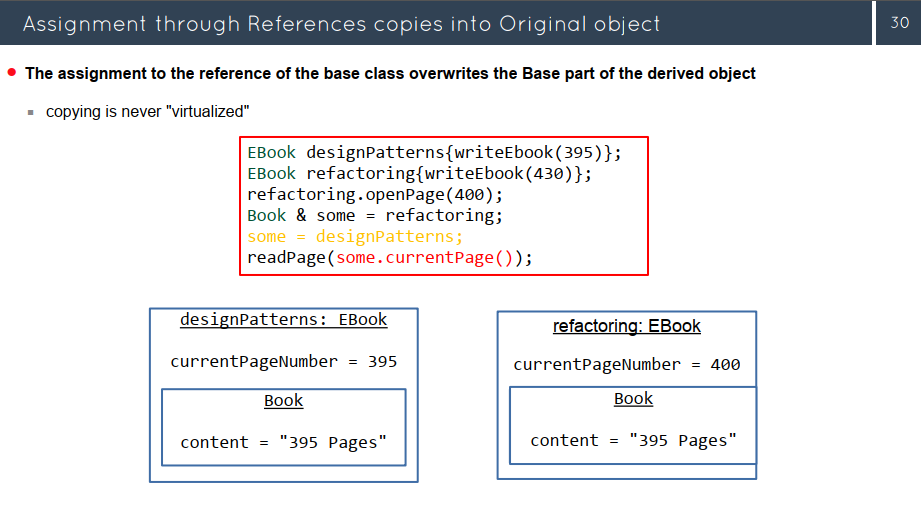
\includegraphics[width=0.9\linewidth]{images/assignment.png}
\section{Histogram}
\begin{lstlisting}[language=C++]
#ifndef HISTOGRAM_H_
#define HISTOGRAM_H_
#include <map>

template<typename T>
struct Histogram {
    void insert (T const key) {
        ++m[key];
    }
    
    unsigned count (T const key) const {
        return m.find(key) != m.end() ? m[key] : 0u;
    }
    // oder
    unsigned count(T const key) const{
		auto result = myMap.find(key);
		if (result == myMap.end()) {
			return 0u;
		} else {
			return result->second;
		}
	}
    
private:
     std::map<T, unsigned> m{};
}
#endif

\end{lstlisting}
\pagebreak
\subsection{HistoramEntry}

\begin{lstlisting}[language=C++]
#ifndef HISTOGRAMENTRY_H_
#define HISTOGRAMENTRY_H_
#include "Word.h"
#include <algorithm>
#include <boost/operators.hpp>
struct HistogramEntry :boost::less_than_comparable<HistogramEntry>, boost::equality_comparable<HistogramEntry> {
	HistogramEntry (Word w, int amount);
	
	inline bool operator <(HistogramEntry const & lhs, HistogramEntry const & rhs) {
		return lhs.amount > rhs.amount;
	}

	inline bool operator >(HistogramEntry const & lhs, HistogramEntry const & rhs) {
		return lhs.amount < rhs.amount;
	}

	inline bool operator ==(HistogramEntry const & lhs, HistogramEntry const & rhs)  {
		return lhs.amount == rhs.amount && lhs.word == rhs.word;
	}
	inline std::ostream& operator<<(std::ostream &out, HistogramEntry const & histogram) {
		histogram.word.print(out);
		out << ": " << histogram.amount;
		return out;
	}
private:
	Word word;
	int amount;
};
#endif /* HISTOGRAMENTRY_H_ */
\end{lstlisting}
\section{Word}
\begin{lstlisting}[language=C++]
#ifndef	WORD_H_
#define	WORD_H_

#include <algorithm>
#include <cctype>
#include <iterator>
#include <string>
#include <ostream>

namespace text {

struct Word {
	Word();
	explicit Word(std::string const & value);
	void read(std::istream &is);
	void print(std::ostream & os) const;

	inline bool operator <(Word const & rhs) const {
		return std::lexicographical_compare(
			std::begin(this->value), std::end(this->value),
			std::begin(rhs.value), std::end(rhs.value),
			[](const char l, const char r) {
				return std::tolower(l) < std::tolower(r);
			}
		);
	}

	inline bool operator ==(Word const & rhs) const {
		return std::equal(
			std::begin(this->value), std::end(this->value),
			std::begin(rhs.value), std::end(rhs.value),
			[](const char l, const char r) {
				return std::tolower(l) == std::tolower(r);
			}
		);
	}

	bool operator>(Word const & other) const {
		return (other < *this);
	}

	bool operator<=(Word const & other) const {
		return !(other < *this);
	}

	bool operator>=(Word const & other) const {
		return !(*this < other);
	}

	bool operator!=(Word const & other) const {
		return !(*this == other);
	}
private:
	std::string value;
	bool isValid(std::string const & value);
};

inline std::istream & operator>>(std::istream & in, Word & word) {
	word.read(in);
	return in;
}

inline std::ostream& operator<<(std::ostream &out, Word const &word) {
	word.print(out);
	return out;
}
}

#endif	/*	WORD_H_	*/
\end{lstlisting}
\begin{lstlisting}[language=C++]
#include "word.h"

#include <iterator>
#include <algorithm>
#include <cctype>
#include <stdexcept>
#include <string>

using text::Word;

Word::Word() : value{"default"} {
}

void Word::read(std::istream &is) {
	if(is.good()) {
		using iter = std::istreambuf_iterator<char>;
		iter input{is};
		iter eof{};
		auto firstChar = std::find_if(input, eof, ::isalpha);
		std::string readWord{};
		std::find_if(firstChar, eof, [&readWord](char c) {
			bool isWordFinished {!std::isalpha(c)};
			if (!isWordFinished) {
				readWord += c;
			}
			return isWordFinished;
		});
		if (isValid(readWord)) {
			value = readWord;
		} else {
			is.setstate(std::ios_base::failbit);
		}
	}
}

Word::Word(std::string const & value) : value { value } {
	if (!isValid(value)) {
		throw std::invalid_argument{"Word isn't valid"};
	}
}

bool Word::isValid(std::string const & value) {
	return !value.empty() && std::all_of(std::begin(value), std::end(value), ::isalpha);
}

void Word::print(std::ostream & os) const {
	os << value;
}
\end{lstlisting}

\section{ENUM}
\begin{lstlisting}[language=C++]
namespace calendar {
    enum class DayOfWeek {
        Mon, Tue, Wed, Thu, Fri, Sat, Sun
    };
}
bool is_weekend(calendar::DayOfWeek day) {
    return day == calendar::DayOfWeek::Sat ||
        day == calendar::DayOfWeek::Sun;
}
\end{lstlisting}

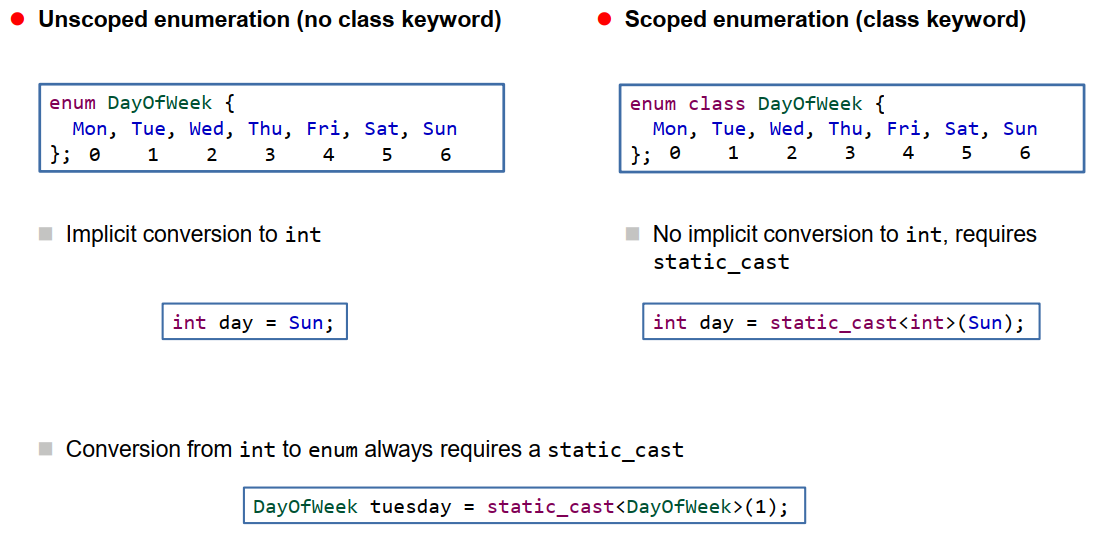
\includegraphics[width=0.9\linewidth]{images/enum.png}
\section{Vectorset}
\begin{lstlisting}[language=C++]
#ifndef VECTORSET_H_
#define VECTORSET_H_
#include <vector>
#include <set>
#include <functional>
#include <algorithm>

template <typename T, typename COMPARE=std::less<T>>
struct vectorset : public std::vector<T> {

   using vectorType = std::vector<T>;
   using vectorType::vectorType;

// Aliases
   using size_type = typename vectorType::size_type;
   using reference = typename vectorType::reference;
   using const_reference = typename vectorType::const_reference;
   using iterator = typename vectorType::iterator;
   using const_iterator = typename vectorType::const_iterator;
   
    vectorset() = default;

    explicit vectorset(std::initializer_list<T> li) : vectorType{li} {
        std::sort(this->begin(), this->end(), COMPARE());
    }

    template <typename ITER>
    vectorset(ITER b, ITER e) : vectorType(b, e) {
       std::sort(this->begin(), this->end(), COMPARE());
    }

    template <typename Elt>
    explicit operator std::multiset<Elt>() const{
    	return std::multiset<Elt>(this->begin(), this->end());
    }

// Functions
   const_iterator find(T const key) const {
        return std::find_if(this->cbegin(), this->cend(), [&key](const T &entry) {
                COMPARE comp{};
                return !comp(key, entry) && !comp(entry, key);
            });
        // return std::find_if(this->cbegin(), this->cend(), [](const T &e) { return e == key; });
        // is equivalent to: return std::find(this->cbegin(), this->cend(), key)
   }

   size_type count(T const key) const {
        return std::count_if(this->cbegin(), this->cend(), [&key](const T &entry) {
                COMPARE comp{};
                return !comp(key, entry) && !comp(entry, key);
        });
   }

   std::multiset<T, COMPARE> asMultiset() {
        return std::multiset<T, COMPARE> (this->cbegin(), this->cend());
   }
};
#endif
\end{lstlisting}

\section{Indexable Set}
\begin{lstlisting}[language=C++]
#ifndef INDEXABLESET_H_
#define INDEXABLESET_H_

#include <set>
#include <stdexcept>
#include <algorithm>

template<typename T, typename COMPARE=std::less<T>>
struct indexableSet	: std::set<T, COMPARE> {
	using container	= std::set<T, COMPARE>;
	using container::container;
	using difference_type = typename container::difference_type;
	using const_reference = typename container::const_reference;

	const_reference	at(difference_type index) const {
		if (index < 0) {
			const long long unsigned int absIndex = abs(index);
			if (absIndex > this->size()) {
				throw std::out_of_range(absIndex + " is out of range");
			}
			return *std::prev(this->cend(), absIndex);
		} else {
			if (static_cast<long long unsigned int>(index) >= this->size()) {
				throw std::out_of_range(index + " is out of range");
			}
			return *std::next(this->cbegin(), index);
		}
	}

	const_reference	operator[](difference_type index) const {
		return this->at(index);
	}

	const_reference	front() const {
		return this->at(0);
	}

	const_reference	back() const {
		return this->at(-1);
	}
};

#endif /* INDEXABLESET_H_ */
\end{lstlisting}

\section{Deck}
\begin{lstlisting}[language=C++]
#ifndef DECK_H
#define DECK_H
#include <deque>
#include <algorithm>
#include <stdexcept>
#include <random>
#include <iterator>

template <typename T>
class Deck {
    using container = std::deque<T>;
    container c;
    using size_type = typename container::size_type;
    using const_iterator = typename container::const_iterator;
    using const_reverse_iterator = typename container::const_reverse_iterator;
    using const_reference = typename container::const_reference;
public:
    Deck() = default;
    explicit Deck(std::initializer_list<T> li) : c{li} {
        this->shuffle();
    }
    template <typename ITER>
    Deck(ITER b, ITER e) : c(b, e) {
        this->shuffle();
    }

    size_type size() const { return c.size(); }
    bool empty() const { return c.empty(); }
    const_reference front() const {
        checkContainer();
        return c.front();
    }

    const_reference back() const {
        checkContainer();
        return c.back();
    }

    void push_back(T const elem) {
        c.push_back(elem);
        shuffle();
    }

    void pop_front() {
        checkContainer();
        c.pop_front();
    }

    void shuffle() {
        std::random_device rd;
        std::mt19937 g(rd());
        std::shuffle(c.begin(), c.end(), g);
    }

    void checkContainer() const {
        if (c.empty()) {
            throw std::out_of_range{"Out of range"};
        }
    }

    // Iteratoren
    const_iterator begin() const { return c.begin(); }
    const_iterator cbegin() const { return c.cbegin(); }

    const_iterator end() const { return c.end(); }
    const_iterator cend() const { return c.cend(); }

    const_reverse_iterator rbegin() const { return c.rbegin(); }
    const_reverse_iterator crbegin() const { return c.crbegin(); }

    const_reverse_iterator rend() const { return c.rend(); }
    const_reverse_iterator crend() const { return c.crend(); }
};
#endif
\end{lstlisting}
\section{Sack}

\subsection{Iterator constructors}
\begin{lstlisting}[language=C++]
void	createSackFromIterators()	{
		std::vector	values{3,	1,	4,	1,	5,	9,	2,	6};
		Sack<int>	aSack{begin(values),	end(values)};
		ASSERT_EQUAL(values.size(),	aSack.size());
}

template	<typename T>
class Sack	{
//...
public:
		template	<typename Iter>
		Sack(Iter	begin,	Iter	end)	:	theSack(begin,	end)	{}
		//...
};
\end{lstlisting}

\begin{lstlisting}[language=C++]
// Retain default constructor
Sack() = default;
\end{lstlisting}

\subsection{Initializer list constructors}

\begin{lstlisting}[language=C++]
Sack(std::initializer_list<T>	values)	: theSack(values)	{}
\end{lstlisting}

\subsection{Extracting a std::vector}
\subsubsection{Usage}
\begin{lstlisting}[language=C++]
//explicit conversion operator
Sack<unsigned>	aSack{1,	2,	3};
auto	values	=	static_cast<std::vector<unsigned>>(aSack);
\end{lstlisting}

\begin{lstlisting}[language=C++]
//member function
Sack<unsigned>	aSack{1,	2,	3};
auto	values	=	aSack.asVector();
auto	doubleValues	=	aSack.asVector<double>();
\end{lstlisting}

\subsubsection{Implementation}

\begin{lstlisting}[language=C++]
//explicit conversion operator
template	<typename Elt>
explicit	operator	std::vector<Elt>()	const	{
		return	std::vector<Elt>(begin(theSack),	end(theSack));
}
\end{lstlisting}

\begin{lstlisting}[language=C++]
//member function
template	<typename Elt	=	T>
auto	asVector()	const	{
		return	std::vector<Elt>(begin(theSack),	end(theSack));
}
\end{lstlisting}

\subsection{Deduction Guide }

\begin{lstlisting}[language=C++]
template	<typename	Iter>
Sack(Iter	begin,	Iter	end)	->	Sack<typename	std::iterator_traits<Iter>::value_type>;
\end{lstlisting}

\subsection{Template Specialization}
\begin{lstlisting}[language=C++]
//Partial Specialization
template <typename T>
struct Sack<T *>;
// Explicit Specialization
template <>
struct Sack<char const *>;
\end{lstlisting}


\section{Espresso}
\subsection{espresso.h}
\begin{lstlisting}[language=C++]
#ifndef ESPRESSO_H_
#define ESPRESSO_H_

#include <iosfwd>
namespace Coffee {

enum class Aroma {
	Cosi, Dharkan, Fortissio, Kazaar, Livanto, Water
};

struct Espresso {
	Aroma aroma{Aroma::Water};

	Espresso() = default;
	explicit Espresso (Aroma aroma);

	bool operator==(Espresso const &other) const;
	bool operator!=(Espresso const &other) const;
	friend std::istream & operator>>(std::istream & in, Espresso & e);


};
}
#endif /* ESPRESSO_H_ */
\end{lstlisting}
\pagebreak
\subsection{espresso.cpp}
\begin{lstlisting}[language=C++]
#include <string>
#include <istream>
#include <map>
#include "espresso.h"

namespace Coffee {

using namespace std::string_literals;

std::map<std::string, Aroma> const aromaNames {
	{"Cosi"s, Aroma::Cosi},{"Dharkan"s, Aroma::Dharkan},
	{"Fortissio"s, Aroma::Fortissio},{"Kazaar"s, Aroma::Kazaar},
	{"Livanto"s, Aroma::Livanto},{"Water"s, Aroma::Water},
};

Espresso::Espresso(Aroma aroma)  : aroma{aroma}{};

bool Espresso::operator ==(Espresso const &other) const {
	return this->aroma == other.aroma;
}

bool Espresso::operator !=(Espresso const &other) const {
	return !(*this == other);
}

std::istream & operator>>(std::istream & in, Espresso & e){
	std::string stringAroma{};
	if (in >> stringAroma) {
		auto const aroma = aromaNames.find(stringAroma);
		if (aroma == aromaNames.end()){
			in.setstate(std::ios_base::failbit);
			return in;
		} else {
			e = Espresso{aroma->second}; // otherwise: e.aroma = aroma->second; 
			return in;
		}
	} else {
		return in;
	}
}
}
\end{lstlisting}

\section{Functor}
\begin{lstlisting}[language=C++]
#include <iostream>
#include <string>
#include <set>
#include <cctype>
#include <iterator>
#include <algorithm>

struct caselessless {
	bool operator()(char const c1, char const c2) const {
		return std::tolower(c1) < std::tolower(c2);
	}
};

void teilB(){
	using namespace std;
	string kasten("OachkatzlSchwoaf");

	set<char, caselessless> s{};

	for (char c : kasten) s.insert(c);

	cout << s.size() << '\n';

	using out = std::ostream_iterator<char>;

	copy(s.begin(), s.end(), out(cout, "."));
}
\end{lstlisting}

% \appendix

% % Code Listings
% \lstlistoflistings

% % List of figures
% \listoffigures

% % List of tables
% \listoftables

% % Bibliography
% \bibliographystyle{plain} 
% \bibliography{literatur}

\end{document}